\documentclass[border=1pt]{standalone}
\usepackage{mathptmx}  % Times text and math
\usepackage{circuitikz}
\usetikzlibrary{arrows.meta}
\ctikzset{bipoles/length=0.75cm, transistors/scale=0.9,
  inductors/coils=4, current/distance=.5, bipoles/diode/height=.32,
  bipoles/diode/width=.26}
\begin{document}
\fontsize{8}{9.6}\selectfont
% dual_loop: control diagram, 1 layout unit = 1 cm (ieee-double)
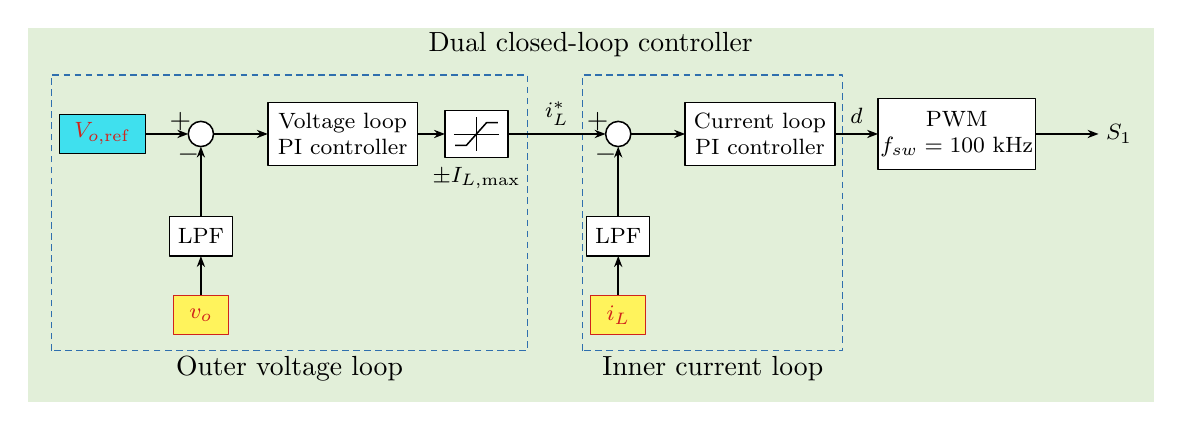
\begin{tikzpicture}[x=1cm, y=1cm, line width=0.55pt, line join=round]
% ---- regions (background) ----
\fill[fill={rgb,255:red,226;green,239;blue,217}] (-0.2,-3.4) rectangle (14.1,1.35);
\node[inner sep=0pt] at (6.95,1.14) {Dual closed-loop controller};
\draw[draw={rgb,255:red,47;green,111;blue,174}, line width=0.44pt, dash pattern=on 2.4pt off 1.6pt] (0.1,-2.75) rectangle (6.15,0.75);
\node[inner sep=0pt] at (3.125,-2.98) {Outer voltage loop};
\draw[draw={rgb,255:red,47;green,111;blue,174}, line width=0.44pt, dash pattern=on 2.4pt off 1.6pt] (6.85,-2.75) rectangle (10.15,0.75);
\node[inner sep=0pt] at (8.5,-2.98) {Inner current loop};
% ---- links ----
\draw[-{Stealth[length=0.14cm]}] (1.3,0) -- (1.84,0);
\draw[-{Stealth[length=0.14cm]}] (2.16,0) -- (2.85,0);
\draw[-{Stealth[length=0.14cm]}] (4.75,0) -- (5.1,0);
\draw[-{Stealth[length=0.14cm]}] (5.9,0) -- (7.14,0);
\draw[-{Stealth[length=0.14cm]}] (7.46,0) -- (8.15,0);
\draw[-{Stealth[length=0.14cm]}] (10.05,0) -- (10.6,0);
\draw[-{Stealth[length=0.14cm]}] (12.6,0) -- (13.4,0);
\draw[-{Stealth[length=0.14cm]}] (2,-2.05) -- (2,-1.55);
\draw[-{Stealth[length=0.14cm]}] (2,-1.05) -- (2,-0.16);
\draw[-{Stealth[length=0.14cm]}] (7.3,-2.05) -- (7.3,-1.55);
\draw[-{Stealth[length=0.14cm]}] (7.3,-1.05) -- (7.3,-0.16);
% ---- vref (tag) ----
\filldraw[fill={rgb,255:red,63;green,224;blue,238}, draw={rgb,255:red,0;green,0;blue,0}, line width=0.33pt] (0.2,-0.25) rectangle (1.3,0.25);
% ---- s1 (sum) ----
\draw[fill=white] (2,0) circle (0.16cm);
% ---- piv (block) ----
\draw[fill=white] (2.85,-0.4) rectangle (4.75,0.4);
% ---- lim (limiter) ----
\draw[fill=white] (5.1,-0.3) rectangle (5.9,0.3);
\draw[line width=0.275pt] (5.212,0) -- (5.788,0) (5.5,-0.216) -- (5.5,0.216);
\draw (5.228,-0.144) -- (5.372,-0.144) -- (5.628,0.144) -- (5.772,0.144);
% ---- s2 (sum) ----
\draw[fill=white] (7.3,0) circle (0.16cm);
% ---- pii (block) ----
\draw[fill=white] (8.15,-0.4) rectangle (10.05,0.4);
% ---- pwm (block) ----
\draw[fill=white] (10.6,-0.45) rectangle (12.6,0.45);
% ---- lpfv (block) ----
\draw[fill=white] (1.6,-1.55) rectangle (2.4,-1.05);
% ---- vo (tag) ----
\filldraw[fill={rgb,255:red,255;green,243;blue,92}, draw={rgb,255:red,208;green,35;blue,28}, line width=0.33pt] (1.65,-2.55) rectangle (2.35,-2.05);
% ---- lpfi (block) ----
\draw[fill=white] (6.9,-1.55) rectangle (7.7,-1.05);
% ---- il (tag) ----
\filldraw[fill={rgb,255:red,255;green,243;blue,92}, draw={rgb,255:red,208;green,35;blue,28}, line width=0.33pt] (6.95,-2.55) rectangle (7.65,-2.05);
% ---- signs ----
\node[inner sep=0pt] at (1.74,0.16) {$+$};
\node[inner sep=0pt] at (1.84,-0.26) {$-$};
\node[inner sep=0pt] at (7.04,0.16) {$+$};
\node[inner sep=0pt] at (7.14,-0.26) {$-$};
% ---- text ----
\node[inner sep=0pt, align=center, font=\fontsize{8}{9.6}\selectfont, text={rgb,255:red,208;green,35;blue,28}] at (0.75,0) {$V_{o,\mathrm{ref}}$};
\node[inner sep=0pt, align=center, font=\fontsize{8}{9.6}\selectfont] at (3.8,0) {Voltage loop\\PI controller};
\node[inner sep=0pt, align=center, font=\fontsize{8}{9.6}\selectfont] at (5.5,-0.56) {$\pm I_{L,\max}$};
\node[inner sep=0pt, align=center, font=\fontsize{8}{9.6}\selectfont] at (9.1,0) {Current loop\\PI controller};
\node[inner sep=0pt, align=center, font=\fontsize{8}{9.6}\selectfont] at (11.6,0) {PWM\\$f_{sw}=100$ kHz};
\node[inner sep=0pt, align=center, font=\fontsize{8}{9.6}\selectfont] at (2,-1.3) {LPF};
\node[inner sep=0pt, align=center, font=\fontsize{8}{9.6}\selectfont, text={rgb,255:red,208;green,35;blue,28}] at (2,-2.3) {$v_{o}$};
\node[inner sep=0pt, align=center, font=\fontsize{8}{9.6}\selectfont] at (7.3,-1.3) {LPF};
\node[inner sep=0pt, align=center, font=\fontsize{8}{9.6}\selectfont, text={rgb,255:red,208;green,35;blue,28}] at (7.3,-2.3) {$i_{L}$};
\node[inner sep=0pt, align=center, font=\fontsize{8}{9.6}\selectfont] at (6.52,0.26) {$i_{L}^{*}$};
\node[inner sep=0pt, align=center, font=\fontsize{8}{9.6}\selectfont] at (10.325,0.23) {$d$};
\node[inner sep=0pt, align=center, font=\fontsize{8}{9.6}\selectfont] at (13.66,0) {$S_{1}$};
\end{tikzpicture}
\end{document}
